\documentclass[a4paper, 12pt]{article} %tipografía y papel

\usepackage[top = 2.5cm, bottom = 2.5cm, left = 2.3cm, right = 2.3cm]{geometry} % margen

\usepackage[T1]{fontenc}
\usepackage[utf8]{inputenc}
\usepackage{geometry} % Page size and margins
\usepackage{amssymb} % Math symbols
\usepackage{amsmath} % Math symbols
\usepackage{amsthm} % Math symbols
\usepackage{empheq} % Math symbols
\usepackage{booktabs} % Tables
\usepackage{setspace} % Spaces
\setlength{\parindent}{0in}
\usepackage[spanish]{babel}
\addto\captionsspanish{\renewcommand{\tablename}{Tabla}}
\usepackage{color} % Colors
\usepackage{bm} % Bold
\usepackage[bb=dsserif]{mathalpha}% Required for inserting images
\usepackage{algorithm} % Pseudocode
\usepackage[noend]{algpseudocode} % Pseudocode
\usepackage{algpseudocode} % Pseudocode
\usepackage{fancyhdr} % Pseudocode
\usepackage{xcolor} % Color
\usepackage{tcolorbox} % Colorbox
\usepackage[framemethod=TikZ]{mdframed} % Colorbox
\usepackage{hyperref}
\numberwithin{figure}{section}
\numberwithin{table}{section}
%% Commands %%
% Boxes
\mdfdefinestyle{definition}{%
    linecolor=teal!20!white,
    roundcorner = 4pt,
    outerlinewidth=1pt,
    innertopmargin=8pt,
    innerbottommargin=8pt,
    innerrightmargin=8pt,
    innerleftmargin=8pt,
    leftmargin = 0pt,
    rightmargin = 0pt,
    backgroundcolor = teal!5!white}

\mdfdefinestyle{theorem}{%
    linecolor=orange!20!white,
    roundcorner = 4pt,
    outerlinewidth=1pt,
    innertopmargin=8pt,
    innerbottommargin=8pt,
    innerrightmargin=8pt,
    innerleftmargin=8pt,
    leftmargin = 0pt,
    rightmargin = 0pt,
    backgroundcolor = orange!5!white}

\mdfdefinestyle{proposition}{%
    linecolor=gray!20!white,
    roundcorner = 4pt,
    outerlinewidth=1pt,
    innertopmargin=8pt,
    innerbottommargin=8pt,
    innerrightmargin=8pt,
    innerleftmargin=8pt,
    leftmargin = 0pt,
    rightmargin = 0pt,
    backgroundcolor = gray!5!white}

\mdfdefinestyle{example}{%
    linecolor=olive!20!white,
    roundcorner = 4pt,
    outerlinewidth=1pt,
    innertopmargin=8pt,
    innerbottommargin=8pt,
    innerrightmargin=8pt,
    innerleftmargin=8pt,
    leftmargin = 0pt,
    rightmargin = 0pt,
    backgroundcolor = olive!5!white}

% Environments
\newcounter{example}[section]
\newenvironment{example}[3]
    {\refstepcounter{example}
    \begin{mdframed}[style=example, nobreak=#1]
        \textbf{Ejemplo \thesection.\theexample}#2. #3
    \end{mdframed}
    }

\newcounter{proposition}[section]
\newenvironment{proposition}[3]
    {\refstepcounter{proposition}
    \begin{mdframed}[style=proposition, nobreak=#1]
        \textbf{Proposición \thesection.\theproposition}#2. #3
    \end{mdframed}
    }

\newenvironment{corolary}[3]
    {\refstepcounter{proposition}
    \begin{mdframed}[style=proposition, nobreak=#1]
        \textbf{Corolario \thesection.\theproposition}#2. #3
    \end{mdframed}
    }

\newcounter{definition}[section]
\newenvironment{definition}[3]
    {\refstepcounter{definition}
    \begin{mdframed}[style=definition, nobreak=#1]
        \textbf{Definición \thesection.\thedefinition}#2. #3
    \end{mdframed}
    }

\newcounter{theorem}[section]
\newenvironment{theorem}[3]
    {\refstepcounter{theorem}
    \begin{mdframed}[style=theorem, nobreak=#1]
        \textbf{Teorema \thesection.\thetheorem}#2. #3
    \end{mdframed}
    }

     %%%%%%%%%% MODIFICAR %%%%%%%%%%
\newcommand{\departamento}{Instituto de Ingeniería Matemática y Computacional }
\newcommand{\ramo}{Taller de Matemáticas Aplicadas (Capstone) }
\newcommand{\sigla}{IMT2116 }
\newcommand{\titulo}{Informe de Medio Semestre }
\newcommand{\semestre}{02 }
\newcommand{\anio}{2025 }
\newcommand{\profe}{Alejandro Cataldo -- Daniel Zúñiga }
\newcommand{\nombre}{Vicente Alfaro, Cristian Chávez, Bruno Parra}

%% Document %%

% \pagestyle{fancy} % With this command we can customize the header style.
% \fancyhf{} 
% \lhead{\footnotesize \sigla - \titulo}
% \rhead{\footnotesize \nombre}
% \cfoot{\footnotesize \thepage}

\begin{document}
\thispagestyle{empty} % This command disables the header on the first page.
\begin{minipage}{2cm}
\vspace{-1.5cm}

\includegraphics[width=2cm]{images/logo.pdf}
\vspace{-1.4cm}
\end{minipage}
\begin{minipage}{\linewidth}
\raggedright \footnotesize
\textsc{Profesor: \profe\\
\sigla - \ramo \\
\departamento}
\end{minipage}
\vspace{0.5cm}

\vspace*{8cm}
\begin{center} 
	{\huge \bf \titulo}\\
	\vspace{2mm}
	{\bf \nombre}\\
        \vspace{1mm}
        {13 de octubre de 2025}
\end{center}
\newpage

\section{Introducción}
\qquad El presente informe de avance corresponde al proyecto de valorización de las opcionalidades de prepago en créditos hipotecarios otorgado por el banco Itaú. Se detallan los avances realizados hasta la fecha, incluyendo el estudio preliminar de los datos, el procesamiento de estos, el análisis exploratorio, los modelos a desarrollar y la planificación de tareas futuras.

\subsection{Contexto Empresa}

\qquad El Banco Itaú Chile es una de las principales instituciones financieras del país y forma parte del grupo Itaú Unibanco, el mayor banco privado de América Latina, con sede en Brasil. En Chile, Itaú inició sus operaciones en 2006, consolidando su presencia tras la fusión con CorpBanca en 2016, lo que lo posicionó entre los bancos más relevantes del sistema financiero nacional.

\qquad El banco ofrece una amplia gama de servicios financieros tanto a personas como a empresas. Sin embargo, aquí nos centramos en su rol de banco de retail, en el cual se centra en ofrecer una diversa variedad de productos y servicios financieros accesibles, como cuentas corrientes, créditos de consumo, hipotecarios, tarjetas de crédito, seguros e inversiones, junto con herramientas digitales que facilitan la gestión cotidiana del dinero.

\subsection{Presentación Problema}

\section{Propósito del Proyecto}
\subsection{Objetivo del Banco}

\qquad El objetivo de la empresa es lograr tener una opción de prepago 
para los créditos hipotecarios. Una opción es un tipo de contrato que da 
el derecho, pero no la obligación, de comprar o vender un activo 
subyacente, que en este caso corresponde al crédito. Es decir, ofrecerle 
al cliente que compre esta opción al banco y así poder prepagar cuando 
el estime conveniente sin que el banco le cobre la clausula de prepago 
mencionada anteriormente.

\qquad Se reconocen tres razones de por qué es relevante que ITAÚ pueda ofrecer este tipo de contratos para sus créditos:

\begin{itemize}
    \item Se podrán ofrecer mejores tasas de interés. El mercado de los 
    créditos hipotecarios es competitivo, por lo que es sumamente 
    valioso poder ajustar al nivel al que se ofrecen los productos. Esto 
    será posible debido a que la opción ya está cubriendo el riesgo del 
    prepago, por lo que no es necesario aplicar la heuristica 
    anteriormente descrita y no elevar innecesariamente las tasas de 
    interés.
    \item Las opciones se pueden aplicar de distintas maneras, esto aumentará considerablemente la variedad de productos que el banco 
    ofrece, ajustándose a las necesidades de cada cliente.
    \item Gestión de riesgos. 
\end{itemize}

\subsection{Propuesta y Objetivo del Proyecto}

\qquad El objetivo principal de este proyecto corresponde a \textbf{valorizar opcionalidades de prepago como una opción del deudor sobre el crédito}. Lo cual, de forma más sencilla, corresponde a cuantificar cuanto le cuesta al banco el prepago del cliente en un tiempo futuro.

\qquad Es por esto que la propuesta de nuestro proyecto es \textbf{calibrar un modelo discreto de tasas para valorizar la opcionalidad de prepago en créditos hipotecarios}. Cuyos detalles se irán describiendo a lo largo de este informe.

\section{Presentación de la metodología}
\subsection{Datos}

\qquad Para tener un valor ajustado para las opciones de prepago, es fundamental conocer el costo de oportunidad que tiene sobre el banco la ejecución de esta acción. Es por esto que nos enfocamos en entender el comportamiento de los instrumentos financieros con los cuales el banco toma posición en el mercado y gestiona riesgos.

\subsubsection{Swap Camara Promedio en CLP}

\qquad Un contrato del tipo \textit{Interest Rate Swap} (IRS) corresponde a un derivado financiero en el que se acuerda un intercambio de flujos a distintas tasas de interes. En este casos nos concentraremos en los contratos interbancarios en CLP, en los cuales un banco entrega un flujo a una tasa fija mientras que la contraparte entrega uno a tasa flotante (variable). El valor del contrato se considera a la tasa fija acordada, lo que se dice pata fija. Estos contratos son la principal manera en la que los bancos pueden gestionar y transferir sus riesgos.

\qquad Actualmente, a nivel nacional, existen 17 tipos de contratos swap transados entre los bancos los cuales son los siguientes:
\begin{table}[H]
\centering

    \begin{tabular}{| c | c |}
    \hline
    Tiempo & Abreviación Bloomberg \\ \hline
    1 mes & CHSWPA \\ \hline
    2 meses & CHSWPB \\ \hline
    3 meses & CHSWPC \\ \hline
    6 meses & CHSWPF \\ \hline
    9 meses & CHSWPI \\ \hline
    1 año & CHSWP1 \\ \hline
    1 año y 6 meses & CHSWP1F \\ \hline
    2 años & CHSWP2 \\ \hline
    3 años & CHSWP3 \\ \hline
    4 años & CHSWP4 \\ \hline
    5 años & CHSWP5 \\ \hline
    7 años & CHSWP7 \\ \hline
    10 años & CHSWP10 \\ \hline
    12 años & CHSWP12 \\ \hline
    15 años & CHSWP15 \\ \hline
    20 años & CHSWP20 \\ \hline
    25 años & CHSWP25 \\ \hline
\end{tabular}
\caption{Los 17 contratos IRS en Chile}\label{fig:tenores}

\end{table}
% \begin{center}
%     {\small Tabla 3.1 - Los 17 contratos IRS en Chile}\\
%     \begin{tabular}{| c | c |}
%     \hline
%     Tiempo & Abreviación Bloomberg \\ \hline
%     1 mes & CHSWPA \\ \hline
%     2 meses & CHSWPB \\ \hline
%     3 meses & CHSWPC \\ \hline
%     6 meses & CHSWPF \\ \hline
%     9 meses & CHSWPI \\ \hline
%     1 año & CHSWP1 \\ \hline
%     1 año y 6 meses & CHSWP1F \\ \hline
%     2 años & CHSWP2 \\ \hline
%     3 años & CHSWP3 \\ \hline
%     4 años & CHSWP4 \\ \hline
%     5 años & CHSWP5 \\ \hline
%     7 años & CHSWP7 \\ \hline
%     10 años & CHSWP10 \\ \hline
%     12 años & CHSWP12 \\ \hline
%     15 años & CHSWP15 \\ \hline
%     20 años & CHSWP20 \\ \hline
%     25 años & CHSWP25 \\ \hline
% \end{tabular}
% \end{center}

\qquad Como ya se dijo anteriormente, entender como se comportarán los valores de estos contratos a futuro es fundamenteal para entender el costo de oportunidad del banco. Y así, poder valorizar opciones de prepago.

\subsubsection{Tasa de Politica Monetaria (TPM)}

\qquad La Tasa de Política Monetaria (TPM) constituye el principal instrumento que utiliza el Banco Central para conducir la política monetaria del país. Se trata de una tasa de interés de referencia que el Banco Central determina con el objetivo de influir en el comportamiento de la economía, especialmente en lo que respecta al control de la inflación y la preservación de la estabilidad de los precios. Esta tasa actúa como una señal para el sistema financiero, ya que sus variaciones inciden directamente en las tasas de interés que aplican los bancos comerciales y otras instituciones financieras en sus operaciones de crédito y ahorro.

\qquad Cuando el Banco Central interviene en el mercado interbancario, es decir, en las transacciones entre bancos, lo hace utilizando la TPM como guía para establecer el costo del dinero en el corto plazo. De esta manera, puede incentivar o desalentar el acceso al crédito, dependiendo de las condiciones económicas que se estén enfrentando. Por ejemplo, si la inflación se encuentra por encima del rango meta establecido, el Banco Central puede optar por elevar la TPM, encareciendo el crédito y reduciendo el consumo y la inversión, lo que tiende a moderar la presión sobre los precios. En cambio, si la economía muestra signos de desaceleración o si la inflación está por debajo del objetivo, puede reducir la TPM para estimular el gasto y la actividad económica. Es por esto que es valioso contar con el historial histórico de la TPM, ya que nos ayudará a analizar los valores de los 17 contratos swap.

\subsubsection{Descripción}

\begin{itemize}
    \item Con respecto a los valores de los contratos IRS, contaremos con el historial del valor de cierre del día para cada tipo, es decir, la tasa fija del último contrato transado ese día. Contamos con el historial desde el 2021 hasta septiembre de 2025, al ser 17 contratos se obtiene una matriz float de tamaño 1256 $\times$ 17. Estos datos los obtenemos de Bloomberg, entregados por la contraparte del banco.
    \item El historial de valores diarios de la TPM es publicada por el Banco Central. Contamos con un historial desde el 2021, lo cual resulta tambien en una matriz float de tamaño 1180 $\times$ 1.
\end{itemize}

\qquad La razón por la cual el historial con el que contamos de ambos datos es desde el 2021, es que en ese año se introducieron los contratos de un mes y dos meses. Por lo que, para que los datos sean comparables necesitamos iniciar desde donde todos los contratos actuales existian.

\subsection{Objetivos Menores}

\qquad A partir de estos datos y de su importancia dentro del proyecto, se reconocen dos nuevos objetivos menores, que siguen siendo relevantes:

\begin{itemize}
    \item Caracterizar la dinámica de la curva swap en pesos chilenos para ser usada en la calibración del modelo.
    \item Alinear el modelo con la estructura de mercado local, con tal que represente fielmente condicones nacionales actuales.
\end{itemize}

\section{Exploración y Procesamiento de los Datos}
\subsection{Normalización}

\subsubsection{Funcionamiento de los Contratos}

\qquad Existe un problema al querer analizar los datos de los valores observados de los contratos, y es que no todos funcionan de la misma manera. Esto es una complicación ya que significa que los datos de la matriz no representan lo mismo con respecto al largo del intervalo de su contrato, haciendo que no sean comparables.

\qquad Las tasas de interés de los contratos de 1 a 18 meses se les dice cero cupón. Esto se debe a que desde el inicio del contrato, solo se hace el intercambio de flujo al finalizar el periodo de tiempo, lo que es el pago del nominal mas los intereses correspondientes.
\begin{figure}[H]
  \centering
      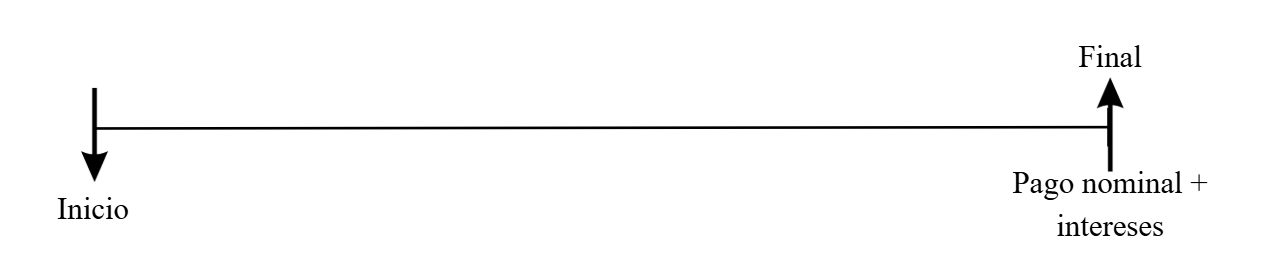
\includegraphics[scale=0.45]{images/diagrama_contratos_cero_cupon.png}
  \caption{Diagrama contratos cero cupón
  }\label{fig:0cupon}
\end{figure}

\qquad Por otro lado, los contratos de 2 a 25 años funcionan con cupones semestrales, es decir, cada seis meses desde el inicio del contrato se hace un depósito de intereses.
\begin{figure}[H]
  \centering
    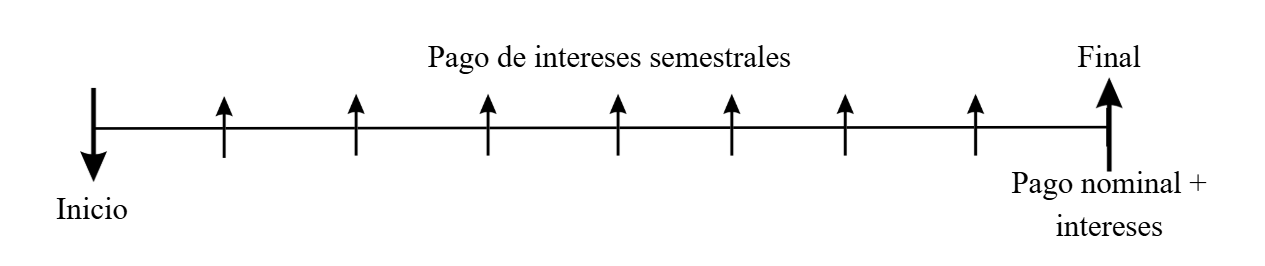
\includegraphics[scale=0.45]{images/diagrama_contratos_semestrales.png}
  \caption{Diagrama contratos con cupones semestrales
  }\label{fig:0cupon}
\end{figure}

\subsubsection{\textit{Bootstrapping}}

\qquad Para solucionar este problema existe un proceso llamado \textit{Bootsraping} financiero. El cual consiste en construir una curva de tasas de cero cupón a partir de los precios de un conjunto de productos con cupones. En otras palabras, para cada contrato que funciona con cupones, queremos encontrar una tasa cero cupón equivalente.

\qquad Para esto utilizamos el factor de descuento, el cual se define de la siguiente manera
$$ \text{DF}(0,T) := \text{El precio hoy de recibir una unidad de dinero en el tiempo } T.$$
Notar que este valor es universal y no depende de los contratos. Sin embargo, es posible saber su valor a través de las tasas de interés de los contratos swap. Para un contrato swap cero cupón a un plazo $T$ y valor $r_T$, el factor de descuento se calcula de la siguiente manera
\begin{equation}
    \text{DF}(0,T) = \dfrac{1}{1 + r_T \frac{\text{buss}(T)}{360}},
\end{equation}
donde $\text{buss}(T)$ es la cantidad de días hábiles en el periodo $T$. Por otro lado, si es que el contrato funcionará con cupones semestrales, el factor de descuento se calcularía así
\begin{equation}
    \text{DF}(0,T) = \dfrac{1 - \sum_{i= 6\text{M}}^{T - 6\text{M}} \frac{\text{buss}(\Delta T_i)}{360} \text{DF}(0, T_i)}{1 + r_T \frac{\text{buss}(\Delta T)}{360}},
\end{equation}
donde $\text{buss}(\Delta T_i)$ corresponde a los días hábiles en tal periodo de 6 meses. Teniendo el factor de descuento, se puede utilizar la ecuación (1) para despejar la tasa cero cupón equivalente, obteniendo así

\begin{equation}
    r_T^{\text{0cupón}} = \dfrac{360}{\text{buss}(T)}\left( \dfrac{1}{\text{DF}(0,T) - 1}\right).
\end{equation}

\qquad Sin embargo, existe un problema. Notar que en la ecuación (2) se es necesario el valor de $\text{DF}(T_i)$ para cada semestre entre el inicio y el final del contrato. Conocer este valor de manera directa no es posible ya que hay $T_i$'s, por ejemplo 30 meses, en los que no existe contrato, por ende no existe una tasa con la cual calcular tal factor de descuento.

\qquad Existen varias formas de resolver este problema, para efectos de esta etapa exploratoria de los datos decidimos realizar una interpolación lineal para la tasa de cada $T_i$ necesario. Por ejemplo, la tasa ficticia para un contrato de 30 meses, con cupones semestrales, se calcula como el promedio entre la tasa de los dos años y tres años.

$$r_{30 \text{M}} = \dfrac{r_{2 \text{Y}} + r_{3 \text{Y}}}{2}.$$

\begin{figure}[H]
    \centering
        \includegraphics[scale=0.45]{images/seriestemporales0cupon.png}
    \caption{Curva de tasas cero cupón
    }\label{fig:0cupon}
\end{figure}
\subsection{PCA}
\qquad Una vez que todos los contratos están normalizados a tasas cero cupón, 
es posible 
comparar los datos entre sí. Sin embargo, sigue existiendo el problema de la 
dimensionalidad. En este caso, cada observación tiene 17 dimensiones, lo que 
hace difícil 
analizar los datos y encontrar patrones. El modelo que utilizaremos recibe 
como input una 
tasa, es por ello que caracterizar los datos en una sola dimensión es 
crucial. 

Litterman y Scheinkman (1991) observaron que con 3 componentes es posible describir el 99\% de la variabilidad observada en el mercado, en particular, la primera componente explica aproximadamente el 96\% de la variabilidad \cite{pca}.

Al realizar PCA obtuvimos que las primeras 2 componentes explican el 98\% de la varianza, pero la primera componente solo explica el 81.5\% de la variabilidad. Este resultado es bajo respecto a lo esperado, pero puede ser explicado por el corto periodo que abarcan los datos, de 2021 a 2025 y por el contexto económico particular de este periodo, que incluye a la pandemia y una alta inflación. 
\begin{figure}[H]
    \centering
        \includegraphics[scale=0.7]{images/pca.png}
    \caption{Varianza explicada por cada componente principal
    }\label{fig:varpca}
\end{figure}
\subsection{La tasa corta}
\qquad A pesar de que la primera componente no explicó de forma esperada la variabilidad de la muestra, podemos interpretar esta componente como la tasa corta (1M), pues esto se debe a fenómenos relacionados al contexto de la muestra y que al variar el nivel de la tasa corta, esta sigue controlando y captura de buena manera el comportamiento de los 17 tenores. En el siguiente gráfico podemos observar la correlación entre la tasa corta (1M) junto a la TPM, notando como la tasa corta sigue de buena manera el comportamiento de la TPM.
\begin{figure}[H]
    \centering
        \includegraphics[scale=0.45]{images/tasacortatpm.png}
    \caption{Tasa corta (1M) vs TPM
    }\label{fig:varpca}
\end{figure}
Por la naturaleza de la TPM, el mercado busca anticiparse a los cambios de la TPM, esto provoca ese efecto “serrucho”, donde la tasa corta (1M) sube antes que la TPM y baja después de la TPM. 

Dado que la tasa corta (1M) explica gran parte de la variabilidad 
de los datos y que tiene sentido económico, se decidió utilizar 
esta tasa para calibrar el modelo.

\section{Modelo Propuesto}
\qquad La teoría de Heath, Jarrow y Morton (HJM) provee un marco general para modelar las tasas de interés. En su enfoque, se describe la dinámica de la curva de tasas de interés de manera estocástica, considerando que las tasas futuras forman un proceso multivariado sujeto a incertidumbre. Esta teoría sirve como base conceptual para modelos de tasas de interés, incluido el modelo de Ho–Lee.

\qquad La idea central dentro de la teoría HJM es modelar la tasa libre de riesgo (o tasa cero cupón) como un proceso de Itô que satisface la ecuación
\begin{equation}
    dr(t) = \mu(r,t)\,dt + \sigma(r,t)\,dW(t),
\end{equation}
donde $\mu$ es el \emph{drift} del modelo, $\sigma$ es la volatilidad instantánea de la tasa $r$ y $W$ es un movimiento browniano estándar.

\subsection{El modelo de Ho--Lee}

\qquad El modelo de Ho--Lee es un caso particular del marco anterior, en el que las tasas de interés a corto plazo se modelan como un proceso estocástico lineal:
\begin{equation}
    dr(t) = \theta(t)\,dt + \sigma\,dW(t),
\end{equation}
donde $r(t)$ es la tasa instantánea en el tiempo $t$, $\theta(t)$ es un término determinista que asegura el ajuste a la curva de tasas inicial, $\sigma$ es la volatilidad constante y $W(t)$ es un movimiento browniano estándar.

\qquad Decir que un mercado es libre de arbitraje significa que no existen oportunidades de obtener una ganancia con inversión neta nula. Bajo este concepto, el modelo de Ho--Lee es libre de arbitraje.

\subsection{Versión discreta del modelo}

\qquad En su versión discreta, el modelo se escribe como
\begin{equation}
    r_{t+\Delta t} = r_t + \theta_t\,\Delta t + \sigma \sqrt{\Delta t}\,\varepsilon_t,
\end{equation}
donde $\varepsilon_t \sim \mathcal{N}(0,1)$ es una variable aleatoria normal estándar (proviene de discretizar el movimiento browniano) y $\Delta t$ es el tamaño del paso temporal. Esta formulación es especialmente útil para simulaciones numéricas y para la valoración de instrumentos financieros en árboles binomiales, como se hizo en este trabajo.

\qquad Con la modelación anterior para $r_{t+\Delta t}$, se generan distintas posibilidades para la tasa en cada paso de tiempo, dando origen a árboles como el de la figura \ref{fig:arbolHL}.

\begin{figure}[h]
    \centering
    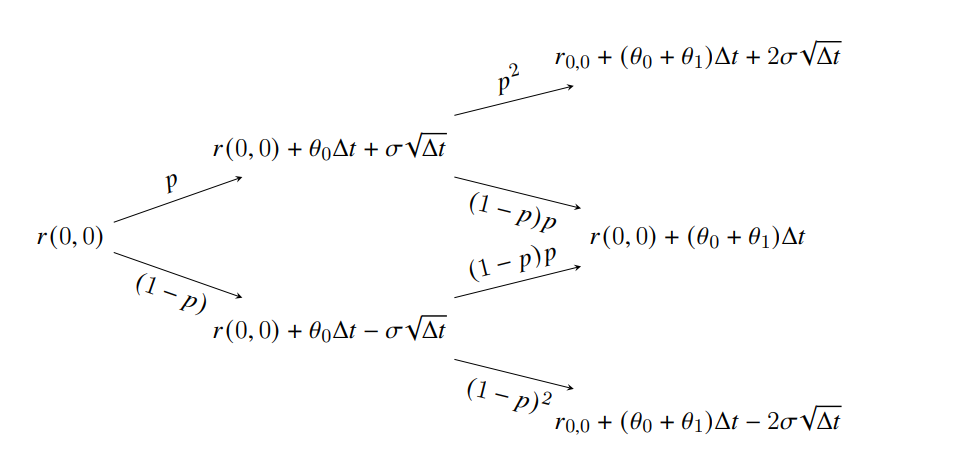
\includegraphics[scale=0.5]{images/grafico_Ho_Lee.png}
    \caption{Ejemplo de árbol generado por el modelo de Ho--Lee.}
    \label{fig:arbolHL}
\end{figure}
\paragraph{Pros de la versión discreta:}
\begin{itemize}
    \item Facilita la implementación computacional, especialmente para bonos y derivados, además de reducir los tiempos de cómputo.
    \item Permite integrar datos de mercado de manera directa y generar árboles de tasas consistentes con la curva inicial.
\end{itemize}

\qquad El uso de este árbol para la valoración de créditos corporativos consiste en calcular el valor del crédito en cada nodo del árbol a partir de las trayectorias de la tasa de interés. El siguiente paso es traer estos valores a presente usando la tasa vigente hasta la fecha del nodo. Luego se estima la esperanza del valor del crédito como el promedio de los valores presentes del crédito en todos los nodos.

\qquad Con base en el procedimiento anterior, se puede ajustar la tasa de interés que se ofrece al cliente en el tiempo inicial para que el retorno promedio de la institución financiera sea el deseado. Esta herramienta permite considerar créditos a distintos plazos, cortando el árbol cuando $t+n\Delta t$ (con $n$ el número de pasos temporales) alcanza el plazo de interés, y a partir de ello realizar los cálculos.


\section{Planificación de Tareas Futuras}

\subsection{Carta Gantt}
\begin{figure}[H]
    \centering
    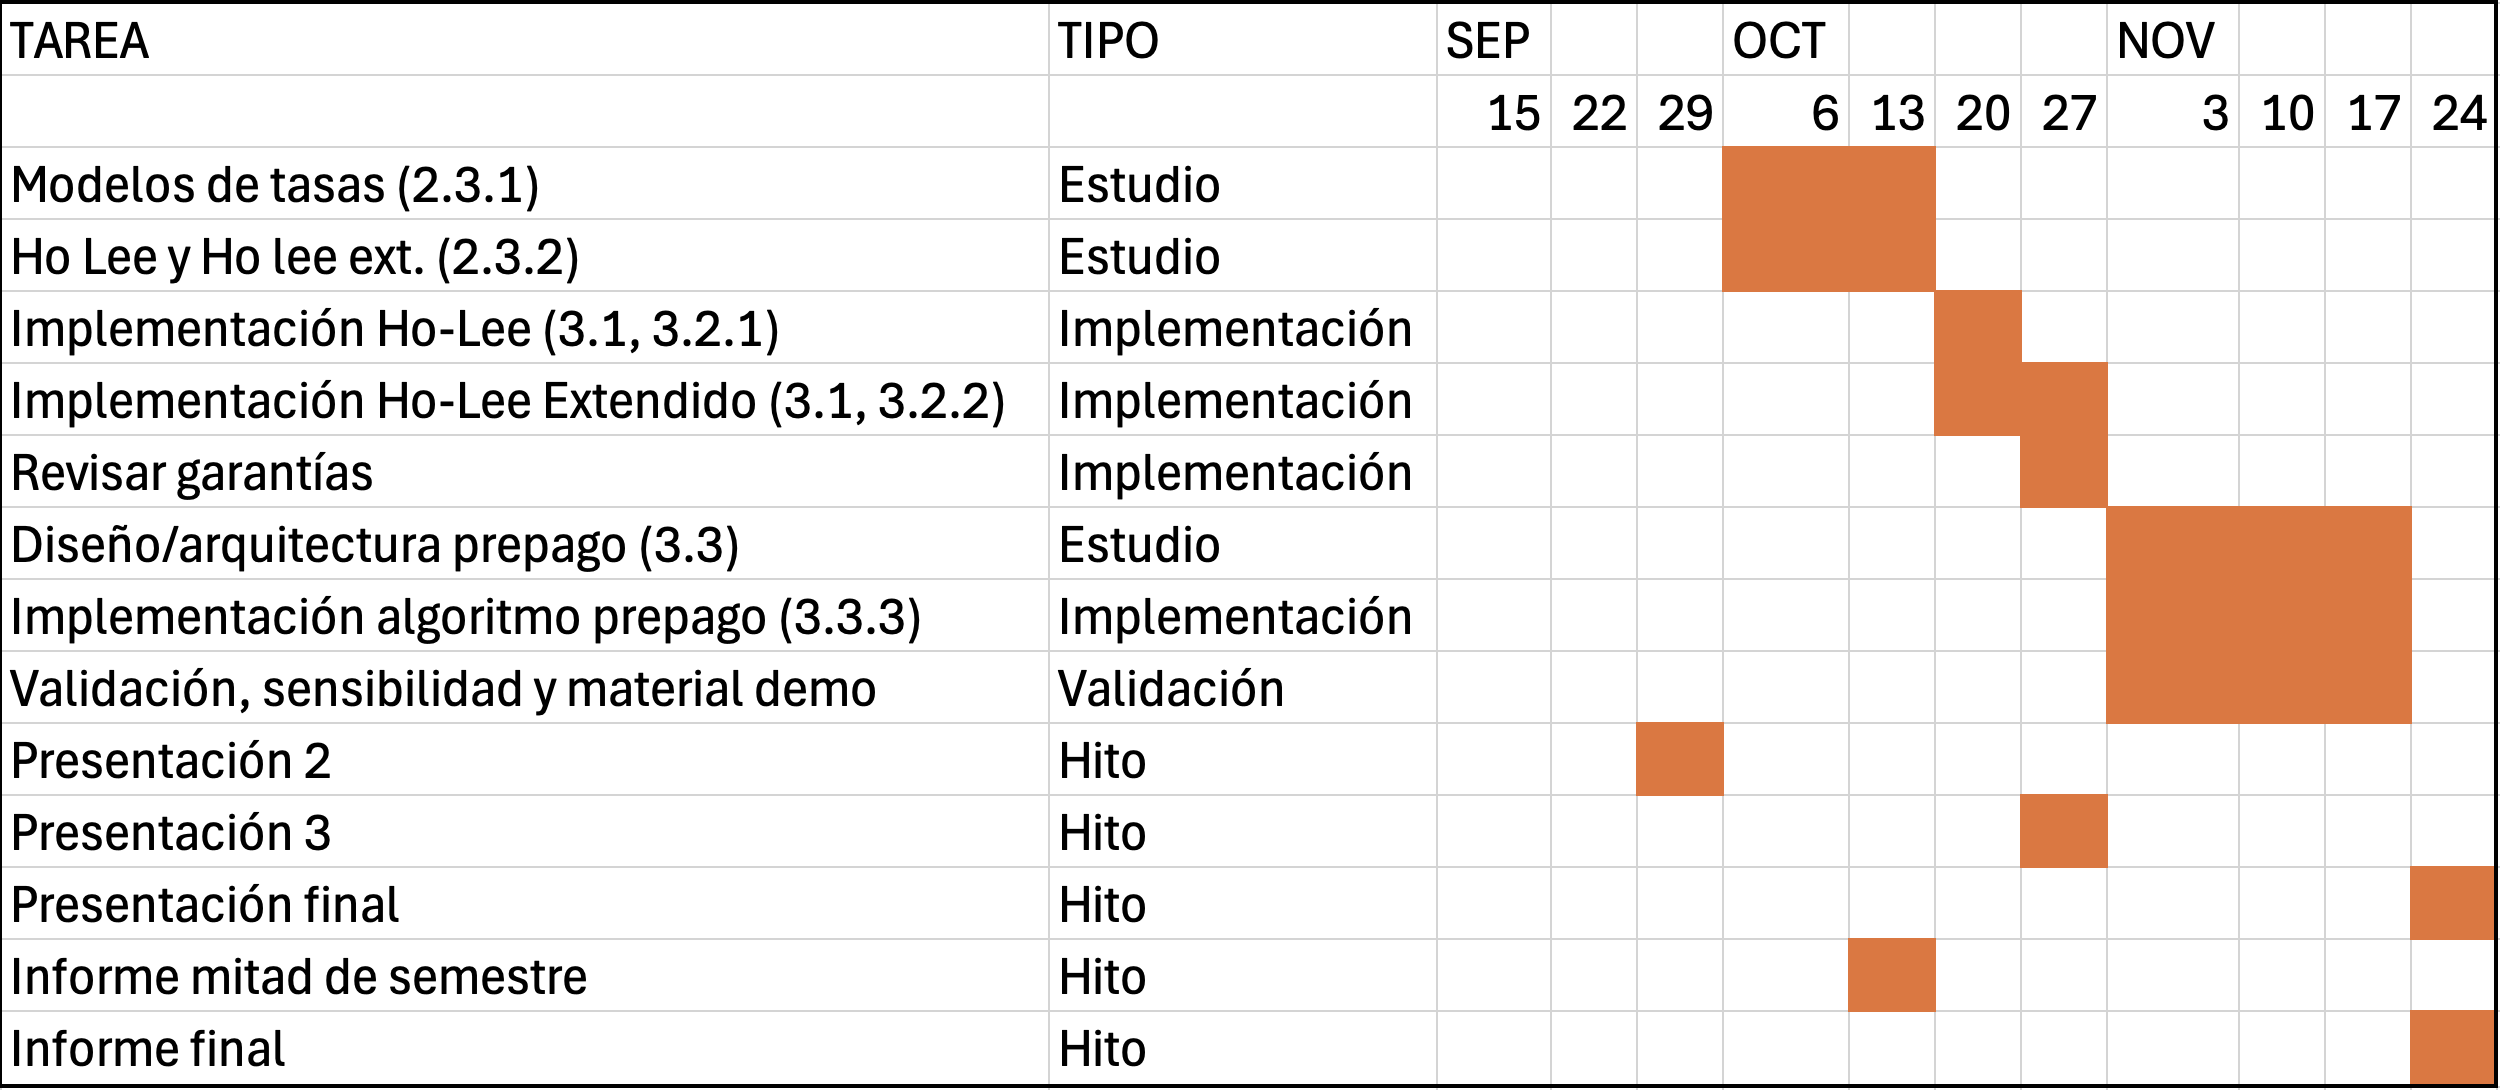
\includegraphics[width=0.9\textwidth]{images/gantt.png}
    \caption{Diagrama de Gantt del proyecto.}
    \label{fig:gantt}
\end{figure}

\subsection{Entregables}

Los entregables fueron acordados con la contraparte del banco considerando los objetivos del proyecto.
\begin{itemize}
    \item Paquete de datos para la calibración del modelo, curvas 0 cupón de las curvas swap cámara peso.
    \item Notebook reproducible con el modelo de Ho-Lee extendido calibrado al set de datos anteriores.
    \item Informe técnico de cómo usar este modelo y límites de aplicación.
\end{itemize}


\newpage
\begin{thebibliography}{1}

\bibitem{pca}
Litterman, R., \& Scheinkman, J. (1991).
\newblock Common factors affecting bond returns.
\newblock \emph{The Journal of Fixed Income}, \emph{1}(1), 54--61.
\newblock \href{https://jfi.pm-research.com/content/1/1/54}{Link}.
\bibitem{valdes}
Valdés, F. (15 de julio de 2004).
\emph{SBIF imparte instrucciones referidas al prepago de créditos.
Se modifica el título I del Capítulo 7{-}1 de la Recopilación Actualizada de Normas}.
Superintendencia de Bancos e Instituciones Financieras (Chile). \href{https://sbif.cl/sbifweb/servlet/Noticia?indice=2.1&idContenido=1870#:~:text=Las%20nuevas%20disposiciones%20legales%20contenidas,trat%C3%A1ndose%20de%20operaciones%20no%20reajustables}{Link}.

\end{thebibliography}


\end{document}